\documentclass{article}

\usepackage{amsmath}
\usepackage{amsfonts}
\usepackage{amssymb}
\usepackage{bbm}
\usepackage{graphicx}
\usepackage[margin=1in]{geometry}

\DeclareMathOperator*{\argmax}{arg\,max}
\DeclareMathOperator*{\argmin}{arg\,min}

\begin{document}
\title{Chapter 2 : Multi-Armed Bandits}
\maketitle


\begin{quote}
	The most important feature distinguishing reinforcement learning from other types of learning is that it uses training information that \textit{evaluates} the actions taken rather than \textit{instructs} by giving correct actions.
\end{quote}

\begin{itemize}
	\item Evaluative feedback indicates how good the action taken was, but not which action is better (depends entirely on the action)
	\item Instructive feedback indicates which action to take, independently of the taken action. (intependent of the action taken)
\end{itemize}

This chapter : \textbf{RL where we learn to act in only one situation} (nonassociative setting). Towards the end of the chapter, we tackle the associative problem (which action to take in more than one situation)

\section{A k-armed Bandit Problem}

\begin{itemize}
	\item One choice among $k$ different options (or actions)
	\item After each choice, we receive a numerical reward chosen from a stationary probability distribution depending on the action selected.
	\item Goal is to maximize the expected total reward over some time period (\textit{time steps})
\end{itemize}

In this problem, each of the $k$ actions have an expected or mean reward (the \textit{value} of the action). Action selected at time $t$ is $A(t)$, and corresponding reward is $R(t)$. Then, the expected reward $q_*(a)$ is given by :

\begin{equation}
q_*(a) \doteq \mathbb{E}\left[ R_t | A_t = a \right]
\end{equation}

This is a trivial problem if we know the value of each action. We assume we don't know them, but we may have estimates ($Q_t(a)$). We would like  $Q_t(a)$ to be close to $q_*(a)$.

If we maintain the estimates at each time step, we have one action with largest estimated reward, which we call the \textit{greedy action}. When selecting them, we are \textbf{exploiting} the current knowledge. If we select another one, we are \textbf{exploring} the system.

Ways to balance between exploration and exploitation might be complicated. Here, we focus only on simple approaches.

\section{Action-value Methods}

Ways to evaluate values of actions. One natural way to etimate it is average of rewards actually received :

\begin{equation}
Q_t(a) \doteq \frac{\text{sum of rewards when } a \text{ taken prior to } t}{\text{number of times } a \text { taken prior to } t} = \frac{\sum_{i=1}^{t-1} R_i \cdot \mathbbm{1}_{A_i=a}}{\sum_{i=1}^{t-1} \mathbbm{1}_{A_i = a}}
\end{equation}

Note that if the denominator is 0, then we define a default value. As the denominator goes to infinity, the LLN says that $Q_t(a)$ converges to $q_*(a)$. This is called the \textbf{sample-average method}. (Maybe not the best method, but simple enough for now).

Simplest action selection rule is to select one of the highest estimated values (greedy).

\begin{equation}
A_t \doteq \argmax_a Q_t(a)
\end{equation}

This focusses on exploitation and not exploration. Simple approach to also do exploration would be to sample greedily most of the time, but sometimes (e.g. with probability $\epsilon$) select an action at random (called $\epsilon$\textit{-greedy} methods)

\begin{quote}
	\textbf{Exercise 2.1} In $\epsilon$\textit{-greedy} action selection, for the case of two actions and $\epsilon=0.5$, what is the probability that the greedy action is selected?
	
	Answer : 0.75 (half of the time, we select the greedy, the other half, we select one action at random, so 50\% of these times (25\% of all times), we select the greedy also)
\end{quote}

\section{The 10-armed Testbed}

In this section, they test 2000 randomly generated k-armed bandit problems with $k=10$. For each problem, they choose $q_*(a)$ using normal distribution with mean 0 and variance 1. Then, actual reward was sampled from a gaussian of variance 1 and mean sampled earlier.

See code I wrote to solve the problem. Results are the same as in the book.

\begin{figure}[ht]
\centering
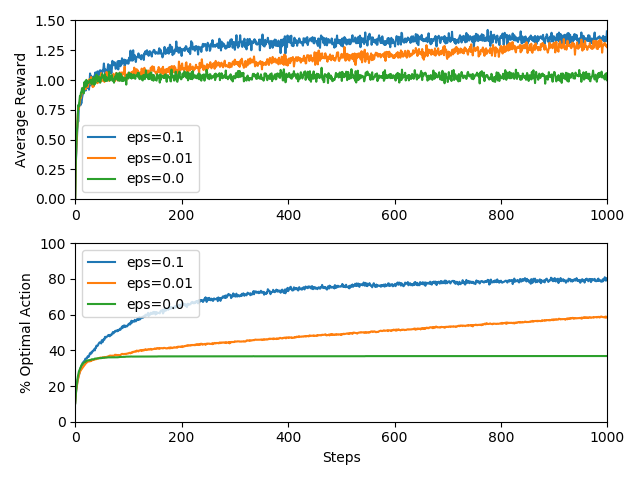
\includegraphics[width=.8\textwidth]{figures/results.png}
\end{figure}

The lower $\epsilon$ will get better over time since it guesses less, but it will learn a lot slower. What we can do is also vary the epsilon with time to have faster convergence.

If the reward variance is larger, this technique does not perform as well also. But even if variance is 0 (reward is expected reward), then exploration might be good in other settings like nonstationary ones (reward values change over time).

\begin{quote}
	
\textbf{Exercise 2.2 : Bandit Example} Consider a k-armed bandir problem with $k=4$ actions, denoted 1,2,3,4. Consider applying to this problem a bandit algorithm using $\epsilon$-greedy action selection, sample-average action-value estimates, and initial estimates of $Q_1(a)=0$, for all $a$. Suppose the initial sequence of actions and rewards is $A_1=1$, $R_1=1$, $A_2=2$, $R_2=1$, $A_3=2$, $R_3=2$, $A_4=2$, $R_4=2$, $A_5=3$, $R_5=0$. On some of these time steps the $\epsilon$ case may have occured, causing an action to be selected at random. On which steps did this definitely occur? On which steps could this possibly have occured?

Answer : Definitely : 2, 5.
Possibly : 1, 3, 4.

\end{quote}

\begin{quote}
\textbf{Exercise 2.3} In the comparison shown in Figure 2.2, which method will perform best in the long run in terms of cumulative reward and probability of selecting the best action? How much better will it be? Express your answer quantitatively.

Answer : Best method will be $\epsilon=0.01$, which will select the optimal action 99.1\% of the time (99\% of the time greedy, 0.1\% random and correct) compared to 91\% for $\epsilon=0.1$ and (undefined) for greedy (depends on the problem). The average reward of the greedy action will always be at $1.$, while the $\epsilon=0.01$ method should cap at an average reward of $\frac{1}{N}\sum_{i=1}^{N} \max(q_*(a) \forall a)$, where $N$ is the number of problems.
\end{quote}


\section{Incremental Implementation}

How to compute with constant memory and constant per-time-step computation? Let's concentrate on a single action to do so. $R_i$ is the reward received after the $i$th selection of this \textit{action}, and $Q_n$ is the estimate of its action value after it has been selected $n-1$ times :

\begin{equation}
Q_n \doteq \frac{1}{n-1}\sum_{i=1}^{n-1} R_i
\end{equation}

Obvious implementation is to maintain a record of all rewards and perform this computation every time, but this is not computationnaly efficient. We can devise an incremental formula instead, so that we can add everything up at every timestep.

\begin{equation}
\begin{split}
Q_{n+1} & = \frac{1}{n}\sum_{i=1}^{n} R_i \\
 & = \frac{1}{n} \left( R_n + \sum_{i=1}^{n-1} R_i \right) \\
 & = \frac{1}{n} \left( R_n + (n-1)\frac{1}{(n-1)} \sum_{i=1}^{n-1} R_i \right) \\
 & = \frac{1}{n} \left( R_n + (n-1)Q_n \right) \\
 & = \frac{1}{n} \left( R_n + nQ_n - Q_n \right) \\
 & = Q_n + \frac{1}{n}\left[ R_n - Q_n \right]
\end{split}
\end{equation}

This implementation only needs to save in memory $Q_n$, $n$ and needs to compute only this small computation instead. (already done in our implementation in previous section!) This thus yield this simpler formula (which looks familiar!) : 

\begin{equation}
\text{NewEstimate} \leftarrow \text{OldEstimate} + \text{StepSize} \left[ \text{Target} - \text{OldEstimate} \right]
\end{equation}

In sum, we update the new estimate with the old estimate and a certain \textit{error estimate} (second term), weighted by a step size.

Note that the step-size parameter changes from timestep to timestep, so it's a bit different from a learning parameter.

\end{document}